\documentclass[handout,instructornotes]{ximera}
%handout:  for handout version with no solutions or instructor notes
%handout,instructornotes:  for instructor version with just problems and notes, no solutions
%noinstructornotes:  shows only problem and solutions

%% handout
%% space
%% newpage
%% numbers
%% nooutcomes

%I added the commands here so that I would't have to keep looking them up
%\newcommand{\RR}{\mathbb R}
%\renewcommand{\d}{\,d}
%\newcommand{\dd}[2][]{\frac{d #1}{d #2}}
%\renewcommand{\l}{\ell}
%\newcommand{\ddx}{\frac{d}{dx}}
%\everymath{\displaystyle}
%\newcommand{\dfn}{\textbf}
%\newcommand{\eval}[1]{\bigg[ #1 \bigg]}

%\begin{image}
%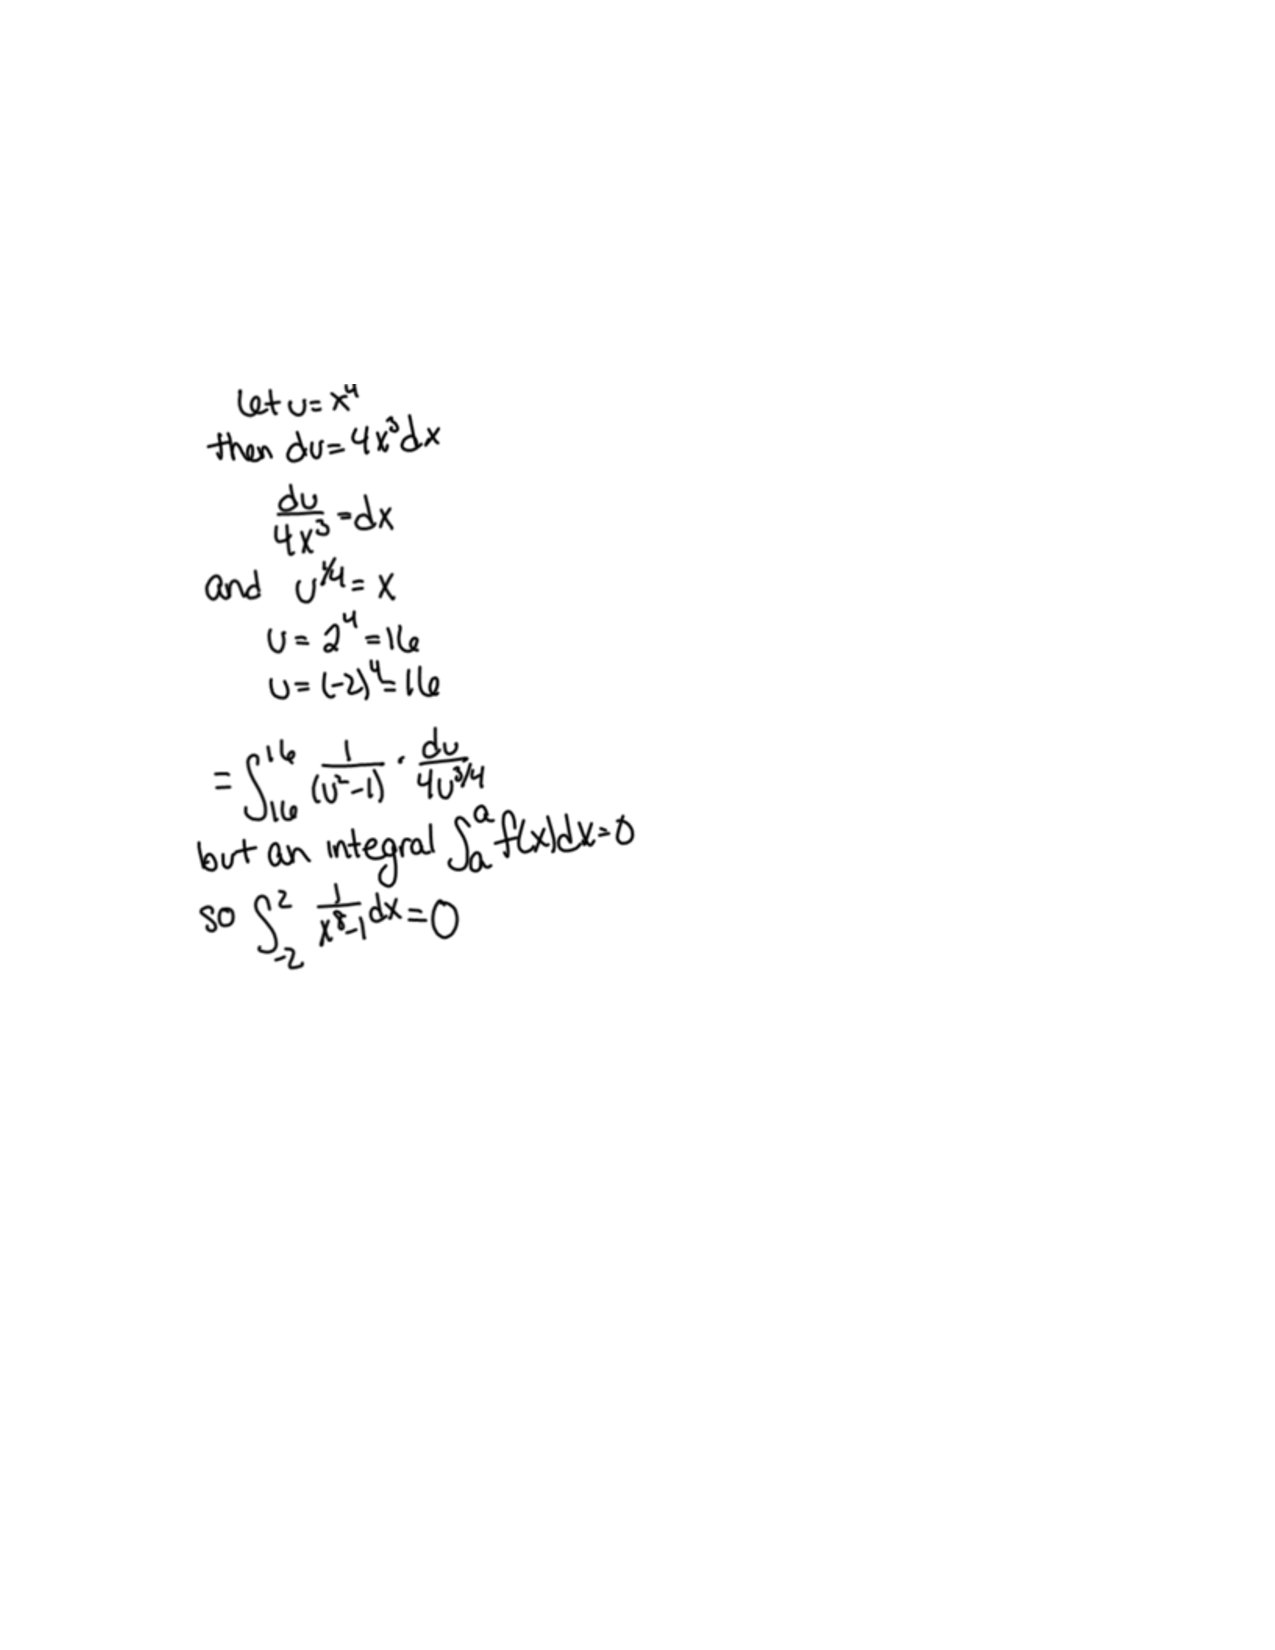
\includegraphics[trim= 170 420 250 180]{Figure1.pdf}
%\end{image}

%add a ``.'' below when used in a specific directory.
\newcommand{\RR}{\mathbb R}
\renewcommand{\d}{\,d}
\newcommand{\dd}[2][]{\frac{d #1}{d #2}}
\renewcommand{\l}{\ell}
\newcommand{\ddx}{\frac{d}{dx}}
\newcommand{\dfn}{\textbf}
\newcommand{\eval}[1]{\bigg[ #1 \bigg]}

\usepackage{multicol}

\renewenvironment{freeResponse}{
\ifhandout\setbox0\vbox\bgroup\else
\begin{trivlist}\item[\hskip \labelsep\bfseries Solution:\hspace{2ex}]
\fi}
{\ifhandout\egroup\else
\end{trivlist}
\fi} %% we can turn off input when making a master document

\title{Recitation \#18: Comparison Tests and Alternating Series - Instructor Notes}  

\begin{document}
\begin{abstract}		\end{abstract}
\maketitle



%Comparison Test Problem
\section{Warm up:}
For each of the following, answer {\bf True} or {\bf False}, and explain why.
	\begin{enumerate}
	
	\item  If $a_n \geq 0$ and $\sum_{n=0}^\infty a_n$ converges, then $\sum_{n=0}^\infty a_n^2$ converges.
	
	\item  If $a_n, b_n \geq 0$ and both $\sum_{n=0}^\infty a_n$ and $\sum_{n=0}^\infty b_n$ converge, then $\sum_{n=0}^\infty a_n b_n$ converges. 
	
	\end{enumerate}
	
	\begin{freeResponse}
		\begin{enumerate}
		
		\item  \dfn{True}
		
		Since $\sum_{n=0}^\infty a_n$ converges, $\lim_{n \to \infty} a_n = 0$.  
		So, in particular, there exists an integer $N$ such that $a_k < 1$ for all $k \geq N$.  
		Then for all $k \geq N$, $a_k^2 < a_k$, and therefore we have that
			\[
			\sum_{n=N}^\infty a_n^2 < \sum_{n=N}^\infty a_n.
			\]
		Thus,  by the Comparison Test, $\sum_{n=0}^\infty a_n^2$ is convergent.
		
		
		
		\item  \dfn{True}
		
		Just as in part (a) there exists an integer $N$ such that $a_k < 1$ for all $k \geq N$.  
		Then
			\[
			\sum_{n=N}^\infty a_n b_n < \sum_{n=N}^\infty b_n
			\]
		and thus, by the Comparison Test, $\sum_{n=0}^\infty a_n b_n$ is convergent.
		
		\end{enumerate}
	\end{freeResponse}
	
\begin{instructorNotes}
Show that these series converge formally using the comparison test.
\end{instructorNotes}







\section{Group work:}



%problem 1
\begin{problem}
	\begin{enumerate}
	
	\item  Why can we not use the Comparison test with $\sum_{k=1}^\infty \frac{1}{k^2}$ to show that $\sum_{k=1}^\infty \frac{1}{k^2 - 5}$ converges?
	
	\item  Adjust $\sum_{k=1}^\infty \frac{1}{k^2}$ to show that $\sum_{k=1}^\infty \frac{1}{k^2 - 5}$ converges via the Comparison Test.
	
	\item  Give a convergent series we can use in the Limit Comparison Test to show that $\sum_{k=1}^\infty \frac{1}{k^2 - 5}$ converges.  
	
	\end{enumerate}
	
	\begin{freeResponse}
		\begin{enumerate}
		
		\item  We cannot use the Comparison Test here because 
			\[
			\frac{1}{k^2} < \frac{1}{k^2 - 5}
			\]
		for all $k \geq 1$.  So we would just be showing the the series in question is greater than a series which converges, which does not give us any information.
		
		
		
		\item  Notice that
			\[
			\frac{2}{k^2} > \frac{1}{k^2 - 5}
			\]
		for all $k \geq 4$.  
		Since $\sum_{k=1}^\infty \frac{1}{k^2}$ converges, $\sum_{k=1}^\infty \frac{2}{k^2} = 2 \sum_{k=1}^\infty \frac{1}{k^2}$.  
		Thus, $\sum_{k=1}^\infty \frac{2}{k^2}$ converges.
		
		Therefore, the Comparison Test with $\sum_{k=1}^\infty \frac{2}{k^2}$ shows that $\sum_{k=0}^\infty \frac{1}{k^2-5}$ converges.
		
		
		
		\item  For the Limit Comparison Test, we \dfn{can} use $\sum_{k=1}^\infty \frac{1}{k^2}$.  
			\begin{align*}
			\lim_{k \to \infty} \frac{\frac{1}{k^2-5}}{\frac{1}{k^2}}
			&= \lim_{k \to \infty} \frac{k^2}{k^2-5}  \\
			&= 1.
			\end{align*}
			
		Thus, since $\sum_{k=1}^\infty \frac{1}{k^2}$ converges, by the Limit Comparison Test we know that $\sum_{k=0}^\infty \frac{1}{k^2-5}$ converges.
		
		\end{enumerate}
	\end{freeResponse}

\end{problem}

\begin{instructorNotes}
This problem may be done as a quick whole class discussion.  
For (b), use something like $\frac{2}{k^2}$.  
Be sure to determine for which $k$ the inequality will hold.
\end{instructorNotes}







%problem 2
\begin{problem}
Determine if the following series converge or diverge.
	\begin{multicols}{2}
	\begin{enumerate}
	
	\item  $\sum_{n=0}^\infty \frac{n^2 + 2n + 1}{3n^3+1}$
	
	\item  $\sum_{n=0}^\infty \frac{n^2+2n+1}{3n^4+1}$
	
	\item  $\sum_{n=0}^\infty \frac{\cos^2 n}{n^3+1}$
	
	\item  $\sum_{n=1}^\infty \left[ \left( 1+\frac{1}{n} \right)^2 e^{-n} \right]$
	
	\end{enumerate}
	\end{multicols}
	
	\begin{freeResponse}
		\begin{enumerate}
		
		\item  Use the \dfn{Limit Comparison Test} with $\sum_{n=1}^\infty \frac{1}{n}$.
			\begin{align*}
			\lim_{n \to \infty} \frac{a_n}{b_n}
			&= \lim_{n \to \infty} \frac{n^2+2n+1}{3n^3+1} \cdot \frac{n}{1}  \\
			&= \frac{1}{3}.
			\end{align*}
			
		Therefore, since $\sum_{n=1}^\infty \frac{1}{n}$ diverges, by the Limit Comparison Test we know that $\sum_{n=0}^\infty \frac{n^2+2n+1}{3n^3+1}$ diverges.
		
		
		
		\item  Use the \dfn{Limit Comparison Test} with $\sum_{n=1}^\infty \frac{1}{n^2}$.
			\begin{align*}
			\lim_{n \to \infty} \frac{a_n}{b_n}
			&= \lim_{n \to \infty} \frac{n^2+2n+1}{3n^4+1} \cdot \frac{n^2}{1}  \\
			&= \frac{1}{3}.
			\end{align*}
			
		Therefore, since $\sum_{n=1}^\infty \frac{1}{n^2}$ converges, by the Limit Comparison Test we know that $\sum_{n=0}^\infty \frac{n^2+2n+1}{3n^4+1}$ converges.
		
		
		
		\item  Use the \dfn{Comparison Test} with $\sum_{n=1}^\infty \frac{1}{n^3}$.  
		
		Since we always have that $0 < \cos^2(n) < 1$, we know that
			\[
			\frac{\cos^2(n)}{n^3 + 1} \leq \frac{1}{n^3+1} < \frac{1}{n^3}.
			\]
		Therefore, by the Comparison Test, we have that $\sum_{n=0}^\infty \frac{\cos^2 n}{n^3+1}$ converges.
		
		
		
		\item  Use the \dfn{Comparison Test} with $\sum_{n=1}^\infty 2 \cdot e^{-n}$.
		
		First, notice that for all $n \geq 3$,
			\[
			\left( 1 + \frac{1}{n} \right)^2 < 2.
			\]		
		Also, notice that $\sum_{n=1}^\infty e^{-n}$ is a convergent geometric series.  
		Therefore $\sum_{n=1}^\infty 2 \cdot e^{-n}$ converges, and so $\sum_{n=1}^\infty \left[ \left( 1+\frac{1}{n} \right)^2 e^{-n} \right]$ converges by the Comparison Test.
		
		\end{enumerate}
	\end{freeResponse}

\end{problem}

\begin{instructorNotes}
These are all done using either the Comparison Test or the Limit Comparison Test.  
Parts (a) and (b) should be done with the limit comparison test (explain why).  
It is important to compare and contrast these two problems.  
Parts (c) and (d) should be done with the Comparison Test (again, explain why).  
The $e^{-n}$ should be treated as a geometric series.
\end{instructorNotes}








%Problem 3
\begin{problem}
Determine if the following series absolutely converge, conditionally converge, or diverge.
	\begin{multicols}{3}
	\begin{enumerate}
	
	\item  $\sum_{n=0}^\infty \frac{(-1)^n}{n+3}$
	
	\item  $\sum_{n=1}^\infty \frac{(-1)^n (n+1)^n}{(2n)^n}$
	
	\item  $\sum_{n=1}^\infty (-1)^{n+1} n^2 e^{\frac{-n^3}{3}}$
	
	\item  $\sum_{n=0}^\infty \frac{(-1)^n \cdot 5}{3^n + 3^{-n}}$
	
	\item  $\sum_{n=4}^\infty \frac{(-2)^n}{n}$
	
	\end{enumerate}
	\end{multicols}
	
	\begin{freeResponse}
	
	\begin{enumerate}
	
	\item  Since $\frac{1}{n+3}$ is positive and decreasing, the Alternating Series Test applies.  
	Thus, this series converges.  
	But we know that $\sum_{n=1}^\infty \frac{1}{n+3}$ diverges (Harmonic Series) and so $\sum_{n=0}^\infty \frac{(-1)^n}{n+3}$ is {\color{red}conditionally convergent}.
	
	\item  Let $a_n = \frac{(n+1)^n}{(2n)^n}$.  
	Applying the Root Test, we see that
		\begin{align*}
		\lim_{n \to \infty} \sqrt[n]{a_n} &= \lim_{n \to \infty} \frac{n+1}{2n}  \\
		&= \frac{1}{2} < 1.
		\end{align*}
	So $\sum_{n=1}^\infty \frac{(n+1)^n}{(2n)^n}$ converges, and therefore $\sum_{n=1}^\infty \frac{(-1)^n (n+1)^n}{(2n)^n}$ is {\color{red}absolutely convergent}.
	
	\item  Let $f(x) = x^2 e^{\frac{-x^3}{3}}$.  
	The function $f(x)$ is continuous, positive, and decreasing.  
	So we apply the integral test
		\begin{align*}
		\int_1^\infty x^2 e^{\frac{-x^3}{3}} \d x
		&= \lim_{b \to \infty} \int_1^b x^2 e^{\frac{-x^3}{3}} \d x  \\
		&= \lim_{b \to \infty} \int_{\frac{1}{3}}^{\frac{b^3}{3}} e^{-u} \d u \qquad {\color{red}u=\frac{x^3}{3}, \, \d u = x^2 \d x}  \\
		&= \lim_{b \to \infty} \left[ -e^{\frac{-b^3}{3}} + e^{\frac{-1}{3}} \right]  \\
		&= 0 + e^{\frac{-1}{3}} = e^{\frac{-1}{3}}.
		\end{align*}
	So, by the Integral Test, $\sum_{n=1}^\infty n^2 e^{\frac{-n^3}{3}}$ converges.  
	Therefore, $\sum_{n=1}^\infty (-1)^{n+1} n^2 e^{\frac{-n^3}{3}}$ is {\color{red}absolutely convergent}.
	
	\item  First, notice that
		\[
		\frac{5}{3^n} > \frac{5}{3^n + 3^{-n}}.
		\]
	Then since $\sum_{n=0}^\infty \frac{5}{3^n}$ converges (geometric series with $r = \frac{1}{3} < 1$), we know that 
	$\sum_{n=0}^\infty \frac{5}{3^n + 3^{-n}}$ converges by the Comparison Test.  
	Thus, the series $\sum_{n=0}^\infty \frac{(-1)^n \cdot 5}{3^n + 3^{-n}}$ is {\color{red}absolutely convergent}.
	
	\item  Since the sequence $\left\{ \frac{(-2)^n}{n} \right\}$ diverges, the series $\sum_{n=4}^\infty \frac{(-2)^n}{n}$ {\color{red}diverges} by the Divergence Test.
	
	\end{enumerate}
	
	\end{freeResponse}
	
\end{problem}

\begin{instructorNotes}
These problems use a mix of tests.  
One of the main goals is for students to get practice determining which test to use.
	\begin{enumerate}
	\item  Limit Comparison Test with the harmonic series
	\item  Root Test
	\item  Integral Test
	\item  Limit Comparison Test
	\item  Divergence Test.  
	Be sure to talk about ``pulling out the $-1$'' to get an alternating series in standard form.  
	Talk about how the Alternating Series Test and the Divergence Test will take care of conditional convergence for most (but not all) alternating series that they will see.
	\end{enumerate}
\end{instructorNotes}







%problem 4
\begin{problem}
\begin{enumerate}

\item  Find an upper bound for how close $\sum_{k=0}^4 \frac{(-1)^k k}{4^k}$ is to the value of $\sum_{k=0}^\infty \frac{(-1)^k k}{4^k}$.

\item  How many terms are needed to estimate $\sum_{n=1}^\infty \frac{(-1)^n \ln n}{n!}$ to within $10^{-6}$?

\end{enumerate}
	\begin{freeResponse}
	\begin{enumerate}

	\item  Recall from the lesson that the remainder $R_n$ is given by
		\[
		R_n = |S - S_n| \leq a_{n+1}.
		\]
	Also notice that
		\[
		\sum_{k=0}^\infty \frac{(-1)^k k}{4^k} = \sum_{k=1}^\infty \frac{(-1)^{k-1} (k-1)}{4^{k-1}}
		\]
	and
		\[
		\sum_{k=0}^4 \frac{(-1)^k k}{4^k} = \sum_{k=1}^5 \frac{(-1)^{k-1} (k-1)}{4^{k-1}}.
		\]
	So
		\begin{align*}
		&\biggr| \sum_{k=0}^\infty \frac{(-1)^k k}{4^k} - \sum_{k=0}^4 \frac{(-1)^k k}{4^k} \biggr|  \\
		&= \biggr| \sum_{k=1}^\infty \frac{(-1)^{k-1} (k-1)}{4^{k-1}} - \sum_{k=1}^5 \frac{(-1)^{k-1} (k-1)}{4^{k-1}} \biggr|  \\
		&= | S - S_5 |  \\
		&= R_6 \leq a_6 = \boxed{\frac{5}{4^5}}
		\end{align*}

	\item  Since $R_n \leq a_{n+1}$, we need to find $n$ so that 
		\begin{align*}
		&a_{n+1} \leq 10^{-6}  \\
		\Longleftrightarrow 	\qquad	&\frac{\ln (n+1)}{(n+1)!} \leq 10^{-6}  \\
		\Longleftrightarrow 	\qquad	&\frac{(n+1)!}{\ln (n+1)} \geq 10^6 
		\end{align*}
	Using a calculator, we see that this inequality holds for $n \approx 8.8$.  
	So for $\boxed{n \geq 9}$, $R_n < 10^{-6}$.  

	\end{enumerate}
	\end{freeResponse}
		
\end{problem}

\begin{instructorNotes}
Split (a) and (b) among the groups.
\end{instructorNotes}









	
	
	
	
	
	
	
	
	

	










								
				
				
	














\end{document} 


















